
\section{\trGenus{} $1$ 的\trCurve}

最后，我们来到了\trGenus{} $1$ 的\trCurve{}这个内容极其丰富的情形。我们将围绕\trDegree{}稳步递增的诸\trLineBundle{}讨论一些有趣的事情，以此来呈现这个理论。虽然眼下这对我们并不特别要紧，但仍请回想：$C$ 上\trDegree{}为 $d$ 的\trLineBundle{}记作 $\mathrm{Pic}^d\,C$（\mbox{定义~18.4.2}）。

\textbf{19.9.1. \trDegree{} $0$ 的\trLineBundle{}（$\mathrm{Pic}^0\,C$）。}

设 $C$ 是一条\trGenus{} $1$ 的\trCurve。那么 $\deg\omega_C=2g-2=0$，而 $h^0(C,\omega_C)=g=1$（由\mbox{练习~19.2.A}）。但带有\trSection{}的\trDegree{} $0$ \trInvertibleSheaf{}唯有\trStructureSheaf{}（\S19.2.4），故我们得出 $\omega_C\cong\OO_C$。（如果你知道\trGenus{} $1$ 的复\trCurve{}都形如 $\mathbb{C}$ 模掉一个\trLattice，而据\mbox{奇迹~18.5.2}，微分层正是\trCanonical{}层，那么你或许并不会惊讶。）

我们转向\trDegree{}更高的\trLineBundle。接下来注意：若 $\deg\mathscr{L}>0$，则\trRiemannRoch{}与\trSerreDuality（\eqref{eq:h0-high-degree}）给出
\[
h^0(C,\mathscr{L})=\deg\mathscr{L}-g+1=\deg\mathscr{L}.
\]

\textbf{19.9.2. \trDegree{} $1$ 的\trLineBundle{}（$\mathrm{Pic}^1(C)$）。}

每个\trDegree{} $1$ 的（$k$-值的）点 $q$ 都决定一个\trLineBundle{} $\OO_C(q)$，而两个互不相同的点决定两个互不相同的\trLineBundle（这是因为一个\trDegree{} $1$ 的\trLineBundle{}在相差纯量倍的意义下只有一个\trSection）。反过来，任一\trDegree{} $1$ 的\trLineBundle{} $\mathscr{L}$ 都形如 $\OO_C(q)$（因为 $\mathscr{L}$ 有一个\trSection——此时只须取它的零点\trDivisor{}即可）。于是，在\trDegree{} $1$ 的\trLineBundle{}与\trDegree{} $1$ 的（闭）点之间，我们便有一个\trCanonical{}的\trBijection。（若 $k$ \trAlgClosed，则由于一切闭点的\trResidueField{}皆为 $k$，这意味着我们在\trDegree{} $1$ 的\trLineBundle{}与闭点之间有一个\trCanonical{}的\trBijection。）

把一条\textbf{\trEllipticCurve}（elliptic curve）定义为一条\trGenus{} $1$ \trCurve{} $E$ 连同一个 $k$-值点 $p$ 的选取。这一点的选取应当永远被看作\trEllipticCurve{}定义的一部分——「椭圆曲线」并不是「\trGenus{} $1$ \trCurve」的同义语。（注意：一条\trGenus{} $1$ 的\trCurve{}完全可以没有任何 $k$-值点！例如，（如 \S19.5.2 中那样）由 $\mathbb{A}^2_{\mathbb{Q}}$ 中的 $y^2=-x^4-1$ 得到的那条超椭圆\trGenus{} $1$ \trCurve\footnote{原书此处作『hypereliptic』，当为『hyperelliptic』之误（脱一 l），径改。——译者注}就没有 $\mathbb{R}$-点，从而也没有 $\mathbb{Q}$-点。当然，若 $k=\bar{k}$，则依\mbox{\trNullstellensatz~3.2.5}，任何闭点都是 $k$-值的。）我们将常常以 $E$ 而非 $C$ 来记\trEllipticCurve。

若 $(E,p)$ 是一条\trEllipticCurve，则在\trDegree{} $0$ \trInvertibleSheaf{}之集（在同构的意义下）与 $E$ 的\trDegree{} $1$ 点之集之间存在一个\trCanonical{}的\trBijection：把诸\trDegree{} $1$ \trLineBundle{}用 $\OO(-p)$ 扭转。具体地，这个\trBijection{}由下式给出
\[
\begin{tikzcd}[row sep=3em]
\mathscr{L} \rar[mapsto] & \operatorname{div}(\mathscr{L}(p)) \\
\OO(q-p) & q. \lar[mapsto]
\end{tikzcd}
\]

但诸\trDegree{} $0$ \trInvertibleSheaf{}（在张量积之下）构成一个\trGroup，于是我们便证明了：

\textbf{19.9.3.\ \trhProposition（\trEllipticCurve{}的\trDegree{} $1$ 点上的群律）。}\ ——\ \emph{上面的\trBijection{}在一条\trEllipticCurve{}的\trDegree{} $1$ 点上定义了一个\trAbelianGroups{}结构，其中 $p$ 是\trIdentityPoint。}

从今往后，我们将不再特别声明地把 $E$ 的闭点与 $E$ 上\trDegree{} $0$ 的\trInvertibleSheaf{}等同起来。

对熟悉复解析图景的人而言，这并不令人惊讶：$E$ 同构于复数模掉一个\trLattice{}所得到的对象：$E\cong\mathbb{C}/\Lambda$。（当然，我们并没有证明这一点。）

\mbox{命题~19.9.3} 目前只是集合之间的一个\trBijection。鉴于 $E$ 具有远为丰富的结构（它有一个\trGenericPoint，并且具有\trVariety{}的结构），这便是一个迹象，表明应当存在某种办法来定义某个概形 $\mathrm{Pic}^0(E)$，而且这应当是一个概形的\trIsomorphism。我们很快就会证明（\mbox{定理~19.10.4}）：$E$ 的\trDegree{} $1$ 点上的这个群结构来自 $E$ 上的一个\trGroupVariety{}结构。

\textbf{19.9.4.}\ \emph{旁注：\trMordell--\trWeil{}定理、群与秩。}\quad 这是一个提一提\trMordell--\trWeil{}定理的好借口：对 $\mathbb{Q}$ 上任何一条\trEllipticCurve{} $E$，$E$ 的 $\mathbb{Q}$-点构成一个\trFinitelyGenerated{}\trAbelianGroups，常称作\trMordell--\trWeil{}群。由有限生成\trAbelianGroups{}的分类定理（主理想整环上有限生成\trModule{}分类的一个特例，\mbox{注记~6.4.4}），$\mathbb{Q}$-点是一个挠部分与一个自由 $\mathbb{Z}$-模的\trDirectSum。这个 $\mathbb{Z}$-模的\trRank{}称为\trMordell--\trWeil{}秩。

\textbf{19.9.5. \trDegree{} $2$ 的\trLineBundle{}（$\mathrm{Pic}^2(E)$）；见图~\ref{fig:genus1-double-cover}。}

注意 $\OO_E(2p)$ 有两个\trSection，故 $E$ 容许 $\mathbb{P}^1$ 的一个二重覆盖（\mbox{练习~19.5.B}）。分歧点之一就是 $p$：$\OO_E(2p)$ 的某个\trSection{}恰在 $p$ 处以 $2$ 阶消失，于是 $\mathbb{P}^1$ 中存在一点，其原像由 $p$ 组成（带重数 $2$）。现在假设 $k=\bar{k}$ 且 $\operatorname{char}k\ne 2$，于是我们可以使用超椭圆\trRiemann--\trHurwitz{}公式（\mbox{定理~19.5.1}），它蕴涵 $E$ 有四个分歧点（$p$ 与另外三个）。反过来，给定 $\mathbb{P}^1$ 中四个点，则恰有一个二重覆盖在这四个点处分支（\mbox{命题~19.5.2}）。于是，椭圆曲线便对应于 $\mathbb{P}^1$ 中四个互不相同的点，其中一点被标记为 $P$，并模掉 $\mathbb{P}^1$ 的\trAutomorphism。等价地，把 $P$ 置于 $\infty$ 处，椭圆曲线便对应于 $\mathbb{A}^1$ 中的三个点，模掉仿射映射 $x\mapsto ax+b$。

\textbf{19.9.A.（练习）}\quad 证明：其余三个分歧点恰好是群律中（非\trIdentityPoint{}的）$2$-挠点。（提示：若其中一点是 $q$，证明 $\OO(2q)\cong\OO(2p)$，但 $\OO(q)$ 不同余于 $\OO(p)$。）

于是（若 $\operatorname{char}k\ne 2$ 且 $k=\bar{k}$），每条\trEllipticCurve{}都恰有四个 $2$-挠点。若你熟悉复图景 $E\cong\mathbb{C}/\Lambda$，这就不足为奇。

\begin{figure}[htbp]
\centering
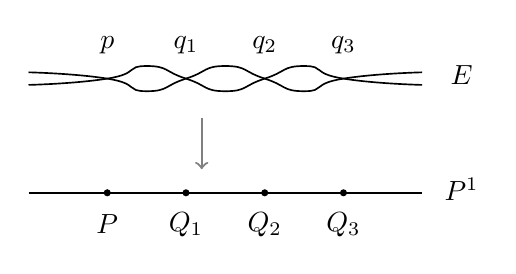
\begin{tikzpicture}[semithick]
  \draw plot[smooth,tension=1] coordinates {(0,0.08) (1,0) (1.5,-0.16) (2,0) (2.5,0.16) (3,0) (3.5,-0.16) (4,0) (5,0.08)};
  \draw plot[smooth,tension=1] coordinates {(0,-0.08) (1,0) (1.5,0.16) (2,0) (2.5,-0.16) (3,0) (3.5,0.16) (4,0) (5,-0.08)};
  \node at (1,0.42) {$p$};
  \node at (2,0.42) {$q_1$};
  \node at (3,0.42) {$q_2$};
  \node at (4,0.42) {$q_3$};
  \node at (5.5,0.05) {$E$};
  \draw[gray,thick,->] (2.2,-0.5) -- (2.2,-1.15);
  \draw (0,-1.45) -- (5,-1.45);
  \fill (1,-1.45) circle (0.045);
  \fill (2,-1.45) circle (0.045);
  \fill (3,-1.45) circle (0.045);
  \fill (4,-1.45) circle (0.045);
  \node at (1,-1.85) {$P$};
  \node at (2,-1.85) {$Q_1$};
  \node at (3,-1.85) {$Q_2$};
  \node at (4,-1.85) {$Q_3$};
  \node at (5.5,-1.4) {$\mathbb{P}^1$};
\end{tikzpicture}
\caption{\trEllipticCurve{}给出射影直线的二重覆盖，在四个点处分支（\S19.9.5）。（依原书手绘图重绘。）}\label{fig:genus1-double-cover}
\end{figure}

\textbf{19.9.6.}\ \emph{后续注记。}\quad 带有\textbf{完全水平 $n$ 结构}（full level $n$ structure）的\trEllipticCurve，是指一条\trEllipticCurve{}连同其 $n$-挠点与 $(\mathbb{Z}/n)^2$ 的一个\trIsomorphism。（若 $n$ 被 $\operatorname{char}k$ 整除，这个概念便会有问题。）于是，带完全水平 $2$ 结构的\trEllipticCurve，与其\trDegree{} $2$ 覆盖描述中给三个其余分支点取定一个排序的\trEllipticCurve，是同一回事。于是（若 $k=\bar{k}$）这些对象由 $\lambda$-直线参数化，我们将在下文讨论它。

\emph{后续的后续。}\quad 带完全水平 $n$ 结构的\trEllipticCurve{}的\trModuliSpace{}这一概念是存在的。这样的\trModuliSpace{}都是\trSmooth{}的\trCurve（在对这句话作恰当解读的意义上——它们是\trStack），并且具有\trSmooth{}的紧化。一个权为 $k$、水平为 $n$ 的\textbf{\trModularForm}（modular form）是 $\omega_M^{\otimes k}$ 的一个\trSection，其中 $\omega_M$ 是这个\trModuliSpace{}的\trCanonical{}层（这个\trModuliSpace{}称作「\textbf{\trModularCurve}」（modular curve））。

\textbf{19.9.7.}\ \emph{\trCrossRatio{}与 $j$-不变量。}\quad （我们保持 $k$ \trAlgClosed{}且特征不为 $2$ 的假设。）若把三个其余的分支点暂时标记为 $Q_1$、$Q_2$、$Q_3\in\mathbb{P}^1$，则有唯一的 $\mathbb{P}^1$ 的\trAutomorphism{}把 $P$、$Q_1$、$Q_2$ 依次送到 $\infty$、$0$、$1$（因为 $\Aut\mathbb{P}^1$ 是 $3$-可迁的，\mbox{练习~15.5.B}）。设在这个映射下 $Q_3$ 被送到某个数 $\lambda$，这里 $\lambda$ 必然不是 $0$、$1$、$\infty$。这个 $\lambda$ 值便称为 $\mathbb{P}^1$ 中四点 $(P,Q_1,Q_2,Q_3)$ 的\textbf{\trCrossRatio}（cross-ratio）（由\trn{Pappus of Alexandria}{亚历山大的帕普斯}所发明，[MO152008]）。

\textbf{19.9.B.（练习）}\quad 证明：$\mathbb{P}^1$ 上四个有序的互不相同的（闭）点（在\trAlgClosedField{} $k$ 上）的同构类，在模掉射影等价（$\mathbb{P}^1$ 的\trAutomorphism）的意义下，由\trCrossRatio{}分类。

\textbf{19.9.C.（练习）}\quad 证明：$(a,b,c,d)$ 的\trCrossRatio{}与 $(b,a,d,c)$ 的\trCrossRatio{}相同。群 $S_4$ 作用在 $\mathbb{P}^1$ 上点的四元组上，从而也作用在它们的\trCrossRatio{}上。证明：$S_4$ 在\trCrossRatio{}上的作用限制到「\trKlein{}四元群」$V_4\subset S_4$ 上时是平凡的。

我们尚未定义\emph{\trModuliSpace}的概念，但上一道练习例示了这样一个事实：$\mathbb{P}^1\setminus\{0,1,\infty\}$（\trCrossRatio{}映射的像）是 $\mathbb{P}^1$ 上四个有序的互不相同点模掉射影等价的\trModuliSpace。

注意：
\begin{itemize}[leftmargin=2.6em,itemsep=2pt,topsep=3pt]
\item 若我们改为把 $P$、$Q_2$、$Q_1$ 送到 $(\infty,0,1)$，则 $Q_3$ 就会被送到 $1-\lambda$。
\item 若我们改为把 $P$、$Q_1$、$Q_3$ 送到 $(\infty,0,1)$，则 $Q_2$ 就会被送到 $1/\lambda$。
\item 若我们改为把 $P$、$Q_3$、$Q_1$ 送到 $(\infty,0,1)$，则 $Q_2$ 就会被送到 $1-1/\lambda=(\lambda-1)/\lambda$。
\item 若我们改为把 $P$、$Q_2$、$Q_3$ 送到 $(\infty,0,1)$，则 $Q_1$ 就会被送到 $1/(1-\lambda)$。
\item 若我们改为把 $P$、$Q_3$、$Q_2$ 送到 $(\infty,0,1)$，则 $Q_1$ 就会被送到 $1-1/(1-\lambda)=\lambda/(\lambda-1)$。
\end{itemize}

于是，这六个值（它们对应于置换 $Q_1$、$Q_2$、$Q_3$ 的对称群 $S_3$）给出同一条\trEllipticCurve，而这条\trEllipticCurve（在对其余三个分支点取定一个排序之后）也将给出这六个值之一。

这已经相当令人满意了。要检验 $k=\bar{k}$ 上的两条\trEllipticCurve{} $(E,p)$ 与 $(E',p')$ 是否\trIsomorphic，我们把二者分别写成在 $p$ 与 $p'$ 处分歧的 $\mathbb{P}^1$ 的二重覆盖，然后给其余分支点排序，再分别计算各自的 $\lambda$（设为 $\lambda$ 与 $\lambda'$），看它们是否由上面六个表达式之一相互联系：
\begin{equation*}\tag{19.9.7.1}\label{eq:cross-ratio-six-values}
\lambda'=\lambda,\ 1/\lambda,\ 1-\lambda,\ 1/(1-\lambda),\ (\lambda-1)/\lambda,\ \text{或}\ \lambda/(\lambda-1).
\end{equation*}

如果代替这个「六值不变量」$\lambda$，存在单个的不变量（就叫它 $j$ 吧），使得 $j(\lambda)=j(\lambda')$ 当且仅当 \eqref{eq:cross-ratio-six-values} 中的等式之一成立，那将会远为方便。这个 $j$-函数想必应当是代数的，因此它会给出一个从 $\lambda$-直线 $\mathbb{A}^1\setminus\{0,1\}$ 到 $j$-直线 $\mathbb{A}^1$ 的映射 $j$。由\mbox{曲线到射影的延拓定理~15.3.1}，它将延拓成一个\trMorphism{} $j\colon\mathbb{P}^1\to\mathbb{P}^1$。由\mbox{练习~16.3.D}，由于这是（对大多数 $\lambda$ 而言）一个 $6$ 对 $1$ 的映射，这个覆盖的\trDegree{}为 $6$（或者更确切地说，至少为 $6$）。

我们可以把这个梦想按如下方式说得更精确。$k$ 上的椭圆曲线对应于 $\mathbb{P}^1\setminus\{0,1,\infty\}$ 的 $k$-值点，并模掉上面给出的 $S_3$ 在 $\lambda$ 上的作用。考虑 $k(\lambda)$ 中被 $S_3$ 固定的子域 $K$。那么扩张 $k(\lambda)/K$ 必然是 \trGalois{}的（例如见 [DF, \S14.2, Thm. 9]），且\trDegree{}为 $6$。我们希望这个子域形如 $k(j)$；若是这样，我们便会得到如上所述的 $j$-映射 $\mathbb{P}^1\to\mathbb{P}^1$。人们可以证明 $K$ 在 $k$ 上\trFinitelyGenerated，然后援引\trLuroth{}定理（我们很快将在\mbox{例~21.4.7}中证明它）；但我们并不需要这个。

不如我们就直接来搜寻这样的 $j$。注意 $\lambda$ 应当在 $k(j)$ 上满足一个六次多项式（或者，更精确地说，按我们此刻所知，满足一个\trDegree{}至少为 $6$ 的多项式），因为对每个 $j$-不变量，一般会有六个 $\lambda$ 值。

正如你毫无疑问已然知晓，这样的 $j$-不变量是存在的。下面就是人人都用的那个 $j$-不变量公式：
\begin{equation*}\tag{19.9.7.2}\label{eq:j-invariant-formula}
j=2^8\,\frac{(\lambda^2-\lambda+1)^3}{\lambda^2(\lambda-1)^2}.
\end{equation*}

你可以轻松验证 $j(\lambda)=j(1/\lambda)=j(1-\lambda)=\cdots$；并且由于 $j$（化成最简分式后）的分子\trDegree{}为 $6$、分母\trDegree{}小于 $6$，$j$ 的确决定了一个从 $\mathbb{P}^1$（以 $\lambda$ 为\trCoordinate）到 $\mathbb{P}^1$（以 $j$ 为\trCoordinate）的\trDegree{} $6$ 映射。但这个看起来很复杂的公式引出了一个问题：这个公式是从哪儿来的？当年的人是怎么想到它的？我们将在很大程度上回答这个问题，不过我们要把 $2^8$ 撇开不谈。正如你所想象的，这个 $2^8$ 来自特征 $2$ 的问题，而为了援引 \S19.5 的结果，我们一直假设 $\operatorname{char}k\ne 2$。（至于为什么在特征 $2$ 下这个 $2^8$ 是被迫加上的，见 [De, p. 64]。而从另一个复解析的视角看，$2^8$ 的由来是因为 $j$ 的 $q$-展开由 $j=q^{-1}+744+\cdots$ 开始：$q^{-1}$ 项的系数为 $1$；见 [Se5, p. 90, Rem. 2]。这两种看似不同的解释由\trTate{}曲线的理论联系在一起；见 [Si2, Thm. V.3.1]。）

与其使用这个白给的公式，不如让我们试着猜一猜 $j$ 是什么。我们不指望得到与 \eqref{eq:j-invariant-formula} 相同的公式，但我们的答案应当与它只相差 $j$-直线（$\mathbb{P}^1$）的一个\trAutomorphism——我们将得到 $j'=(aj+b)/(cj+d)$，其中 $a$、$b$、$c$、$d$ 为某组数（\mbox{练习~15.5.A}）。

我们要寻找某个 $j'(\lambda)$，使得 $j'(\lambda)=j'(1/\lambda)=\cdots$。于是我们想要某个在这个 $S_3$-作用之下不变的、含 $\lambda$ 的表达式。第一种可能的做法是取这六个数的乘积：
\[
\lambda\cdot(1-\lambda)\cdot\frac{1}{\lambda}\cdot\frac{\lambda-1}{\lambda}\cdot\frac{1}{1-\lambda}\cdot\frac{\lambda}{\lambda-1}.
\]
这就傻了，因为乘积显然等于 $1$。

一个好一些的想法是把它们统统加起来：
\[
\lambda+(1-\lambda)+\frac{1}{\lambda}+\frac{\lambda-1}{\lambda}+\frac{1}{1-\lambda}+\frac{\lambda}{\lambda-1}.
\]
这也不行，因为它们加起来是 $3$——这六项两两配对，每对的和都为 $1$。

（你或许会意识到这行不通的另一个理由：如果你审视这个和，你会意识到你将得到「\trDegree{}至多为 $3$」的东西除以「\trDegree{}至多为 $2$」的东西。那么，若 $j'=p(\lambda)/q(\lambda)$，则 $\lambda$ 在 $j$ 上是一个三次式的根。但我们说过 $\lambda$ 应当在 $j'$ 上满足一个六次式。避免矛盾的唯一办法是 $j'\in k$。）

但你毫无疑问马上就会有另一个主意。一个好主意是取这六个根的第二个对称函数。一个等价而更易于徒手演算的做法，是把这六项的平方加起来。甚至在动手计算之前，我们就能看出这招会灵：它显然会产出一个分子与分母\trDegree{}至多为 $6$ 的分式，并且它不是常数——当 $\lambda$ 是某个固定的小的数值（比如说 $1/2$）时，平方和是某个小的实数；而当 $\lambda$ 是一个大的实数时，平方和将不得不是某个大的实数（不同于 $\lambda=1/2$ 时的值）。

当你徒手把这些平方加起来（这并不难）之后，你将得到
\[
j'=\frac{2\lambda^6-6\lambda^5+9\lambda^4-8\lambda^3+9\lambda^2-6\lambda+2}{\lambda^2(\lambda-1)^2}.
\]

的确 $k(j)\cong k(j')$：你可以（再次徒手）验证
\[
2j/2^8=\frac{2\lambda^6-6\lambda^5+12\lambda^4-14\lambda^3+12\lambda^2-6\lambda+2}{\lambda^2(\lambda-1)^2}.
\]

于是 $2j/2^8-j'=3$。

\textbf{19.9.8. \trDegree{} $3$ 的\trLineBundle{}（$\mathrm{Pic}^3(E)$）。}

在 \S19.9.5 关于\trDegree{} $2$ \trLineBundle{}的讨论中，我们为了援引\trRiemann--\trHurwitz{}公式而假设了 $\operatorname{char}k\ne 2$ 与 $k=\bar{k}$。在本小节中，我们将不带任何假设出发，并随需要陆续追加假设。这样你就会看到：在更弱的假设下，哪些部分结果仍然成立。

考虑\trDegree{} $3$ 的\trInvertibleSheaf{} $\OO_E(3p)$。由\trRiemannRoch{}（\eqref{eq:h0-high-degree}），
\[
h^0(E,\OO_E(3p))=\deg(3p)-g+1=3.
\]
由于 $\deg\OO_E(3p)>2g$，这就给出一个\trClosedEmbedding（\mbox{注记~19.2.11}与\mbox{练习~19.2.E}）。于是我们有一个闭嵌入 $E\hookrightarrow\mathbb{P}^2_k$，其像为一条三次\trCurve。此外，$\mathbb{P}^2_k$ 中有一条以重数 $3$ 与 $E$ 相交于点 $p$ 的直线，它对应于 $\OO(3p)$ 的那个恰在 $p$ 处以重数 $3$ 消失的\trSection。（平面内以至少 $2$ 的重数与一条\trSmooth\trCurve{}相交的直线是一条\trTangentLine；见\mbox{定义~13.3.3}。平面内以至少 $3$ 的重数与一条\trSmooth\trCurve{}相交的直线称为一条\textbf{\trFlex{}线}（flex line），而该点便是这条\trCurve{}的一个\textbf{\trFlex{}点}（flex point）或简称\textbf{\trFlex}（flex）。）（见图~\ref{fig:weierstrass-cubic}。）

\begin{figure}[htbp]
\centering
\begin{tikzpicture}[semithick]
  \draw[dotted] (0,0) circle (1.7);
  \node at (-2.5,1.35) {$\mathbb{P}^2$};
  \node at (-2.32,0.88) {（未按比例！）};
  \draw[dotted] (0,-1.7) -- (0,1.7);
  \draw[dotted] (-1.7,0) -- (1.7,0);
  \node at (-0.62,-1.28) {$x=0$};
  \node at (0.98,0.24) {$y=0$};
  \node at (2.2,-1.05) {$z=0$};
  \draw (-1.05,0) ellipse (0.32 and 0.18);
  \draw plot[smooth,tension=1] coordinates {(-0.3,2.02) (0,1.72) (0.32,1.28) (0.16,0.62) (0.06,0.18) (0.18,-0.28) (0.42,-0.9) (0.5,-1.36)};
  \fill (0,1.72) circle (0.04);
  \node at (0.32,1.92) {$p$};
\end{tikzpicture}
\caption{寻找一条\trEllipticCurve{}的\trn{Weierstrass}{魏尔斯特拉斯}三次曲线化身。（依原书手绘图重绘。）}\label{fig:weierstrass-cubic}
\end{figure}

在 $\mathbb{P}^2_k$ 上选取射影\trCoordinate，使得 $p$ 被送到 $[0,1,0]$，而\trFlex{}线正是无穷远线 $z=0$。那么这条三次曲线便呈如下形状：
\[
\begin{aligned}
&?\,x^3\;\;+\;\;0\,x^2y\;\;+\;\;0\,xy^2\;\;+\;\;0\,y^3\\
&+\;\;?\,x^2z\;\;+\;\;?\,xyz\;\;+\;\;?\,y^2z\qquad\qquad\qquad=\ 0.\\
&\qquad+\;\;?\,xz^2\;\;+\;\;?\,yz^2\\
&\qquad\qquad+\;\;?\,z^3
\end{aligned}
\]

$x^3$ 的系数不是 $0$（否则这条三次曲线将被 $z$ 整除）。把整个方程除以这个系数，我们便可设 $x^3$ 的系数为 $1$。$y^2z$ 的系数也不是 $0$（否则这条三次曲线在 $x=z=0$ 处\trSingular）。我们可以缩放 $z$（即把 $z$ 换成它的一个适当的倍数），使得 $y^2z$ 的系数为 $-1$。若 $k$ 的特征不是 $2$，那么我们接着可以把 $y$ 换成 $y+?x+?z$，使得 $xyz$ 与 $yz^2$ 的系数为 $0$；而若 $k$ 的特征不是 $3$，我们便可以把 $x$ 换成 $x+?z$，使得 $x^2z$ 的系数也为 $0$。总之，若 $\operatorname{char}k$ 不是 $2$ 或 $3$，这条\trEllipticCurve{}便可以写成
\begin{equation*}\tag{19.9.8.1}\label{eq:weierstrass-normal-form}
y^2z=x^3+axz^2+bz^3.
\end{equation*}
这称为这条曲线的\textbf{\trWeierstrassNormalForm}（Weierstrass normal form）。

\textbf{19.9.9.}\ \emph{从\trn{Weierstrass}{魏尔斯特拉斯}三次曲线到二重覆盖。}\quad 令 $z=1$，或者更精确地说，在特异开集 $z\ne 0$ 中使用非齐次\trCoordinate{}工作，我们便看到这条曲线的超椭圆（二重覆盖）描述。下面就是三次曲线描述中何以能看见二重覆盖描述的几何解释。从 $p=[0,1,0]$ 出发投射这条三次曲线（见图~\ref{fig:weierstrass-to-double-cover}）。这是一个映射 $E\setminus p\to\mathbb{P}^1$（由 $[x,y,z]\mapsto[x,z]$ 给出），它基本上就是这条三次曲线到 $x$-轴的竖直\trProjection。（图~\ref{fig:weierstrass-to-double-cover}或许有助于你想见这个画面。）由\mbox{曲线到射影的延拓定理~15.3.1}，\trMorphism{} $E\setminus p\to\mathbb{P}^1$\footnote{原书此处作『$E-p$』，当为『$E\setminus p$』之误，径改。——译者注}可延拓到 $p$ 之上。若 $\mathscr{L}:=\OO(3p)$ 是给出这个\trMorphism{} $E\hookrightarrow\mathbb{P}^2$ 的\trLineBundle（经由\mbox{定理~15.2.2}——它以\trLineBundle{}的语言描述到射影空间的映射），那么给出到 $\mathbb{P}^1$ 的映射的那两个\trSection{} $x$ 与 $z$ 分别在 $p$ 处以 $1$ 阶与 $3$ 阶消失。为了把这个\trRationalMap{}「解消」成一个名副其实的\trMorphism，我们把 $x$ 与 $z$ 解释为 $\mathscr{L}(-p)=\OO(2p)$ 的\trSection，于是它们生成一个\trBasePointFree\trLinearSystem，从而生成一个到 $\mathbb{P}^1$ 的\trMorphism。（你或许能把这解读为用另一种语言实现\mbox{定理~15.2.2} 的证明。）类似的想法——施于四次曲线而非三次曲线——曾在\mbox{练习~19.7.C} 中得到使用。

\begin{figure}[htbp]
\centering
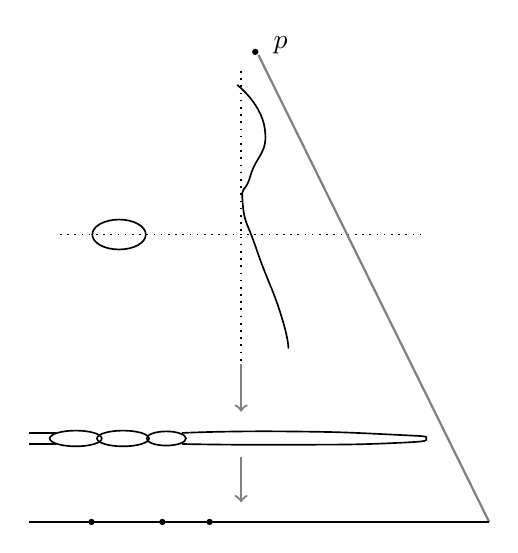
\begin{tikzpicture}[semithick]
  \draw[dotted] (0,-2.5) -- (0,1.2);
  \draw[dotted] (-2.3,-0.9) -- (2.3,-0.9);
  \draw (-1.55,-0.9) ellipse (0.34 and 0.19);
  \draw plot[smooth,tension=1] coordinates {(-0.05,1.0) (0.3,0.45) (0.12,-0.15) (0.02,-0.5) (0.2,-1.1) (0.5,-1.9) (0.6,-2.35)};
  \fill (0.18,1.42) circle (0.04);
  \node at (0.5,1.5) {$p$};
  \draw[gray,thick] (0.22,1.38) -- (3.15,-4.55);
  \draw[gray,thick,->] (0,-2.55) -- (0,-3.15);
  \draw (-2.7,-3.42) -- (-2.35,-3.42);
  \draw (-2.7,-3.56) -- (-2.35,-3.56);
  \draw (-2.1,-3.49) ellipse (0.33 and 0.10);
  \draw (-1.5,-3.49) ellipse (0.33 and 0.10);
  \draw (-0.95,-3.49) ellipse (0.25 and 0.09);
  \draw plot[smooth,tension=1] coordinates {(-0.75,-3.42) (0.5,-3.40) (1.9,-3.44) (2.35,-3.49) (1.9,-3.55) (0.5,-3.57) (-0.75,-3.56)};
  \draw[gray,thick,->] (0,-3.72) -- (0,-4.3);
  \draw (-2.7,-4.55) -- (3.15,-4.55);
  \fill (-1.9,-4.55) circle (0.04);
  \fill (-1.0,-4.55) circle (0.04);
  \fill (-0.4,-4.55) circle (0.04);
\end{tikzpicture}
\caption{从\trn{Weierstrass}{魏尔斯特拉斯}三次曲线到\trEllipticCurve{}的二重覆盖解读（参看图~\ref{fig:weierstrass-cubic}）。（依原书手绘图重绘。）}\label{fig:weierstrass-to-double-cover}
\end{figure}

作为一个推论，只要费上一点汗水，我们就能把 $j$-不变量计算为 $a$ 与 $b$ 的函数：
\[
j(a,b)=\frac{2^8\,3^3\,a^3}{4a^3+27b^2}.
\]

\textbf{19.9.D.（练习）}\quad 证明：这条三次曲线的诸\trFlex{}点恰好是群 $E$ 中的 $3$-挠点。（「\trFlex」的定义见 \S19.9.8：它是切线与曲线在该点以至少 $3$ 的重数相交的那个点。事实上，若 $k$ \trAlgClosed{}且 $\operatorname{char}k\ne 3$，它们共有九个。如果你熟悉复数的故事——$E\cong\mathbb{C}/\Lambda$——这不会令你惊讶。）

\textbf{19.9.10. 群律，几何地。}

这个群律有一个借助\trn{Weierstrass}{魏尔斯特拉斯}形式的优美的经典描述。参看图~\ref{fig:group-law-geometric}。在\trn{Weierstrass}{魏尔斯特拉斯}\trCoordinate{}下，原点 $p$ 是 $E$ 与无穷远线（$z=0$）相交的唯一一点；事实上，无穷远线对应于 $\OO(3p)$ 的重言截面。若一条直线与 $E$ 相交于三点 $p_1$、$p_2$、$p_3$，则
\[
\OO(p_1+p_2+p_3)\cong\OO(3p),
\]
从而（在群律中）$p_1+p_2+p_3=0$。

于是，为求一个点 $s$ 的逆，我们考虑 $E$ 与直线 $\overline{sp}$ 的交：$-s$ 就是第三个交点。为求两点 $q$ 与 $r$ 的和，我们考虑 $E$ 与直线 $\overline{qr}$ 的交，并把第三个交点称为 $s$。然后我们通过把 $s$ 与 $p$ 相连来计算 $-s$，从而得到 $q+r$。

\begin{figure}[htbp]
\centering
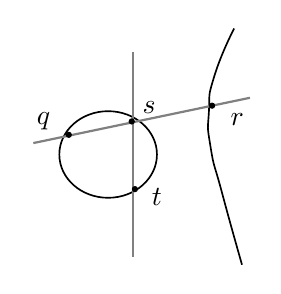
\begin{tikzpicture}[semithick]
  \draw (0,0) ellipse (0.62 and 0.55);
  \draw plot[smooth,tension=1] coordinates {(1.6,1.6) (1.35,1.0) (1.28,0.55) (1.3,0.1) (1.45,-0.5) (1.7,-1.4)};
  \draw[gray,thick] (0.32,-1.3) -- (0.32,1.3);
  \draw[gray,thick] (-0.95,0.145) -- (1.8,0.72);
  \fill (-0.5,0.25) circle (0.04);  \node at (-0.82,0.42) {$q$};
  \fill (0.30,0.42) circle (0.04);  \node at (0.52,0.60) {$s$};
  \fill (1.32,0.62) circle (0.04);  \node at (1.64,0.44) {$r$};
  \fill (0.34,-0.44) circle (0.04); \node at (0.62,-0.54) {$t$};
\end{tikzpicture}
\caption{\trEllipticCurve{}上的群律，几何地。（依原书手绘图重绘。）}\label{fig:group-law-geometric}
\end{figure}

我们可以把关于\trWeierstrassNormalForm{}中三次曲线之群律的这一番描述讲给任何熟悉射影空间概念与群概念的人听，但那样一来，我们就必须证明我们所给出的构造确实定义了一个群。特别地，我们将不得不证明结合律，而这并不是先验清楚的。但在眼下这个情形，我们已经通过给出到 $\mathrm{Pic}^0E$ 的一个\trBijection{}确立了\trDegree{} $1$ 点构成一个群，我们不过是在解读 $\mathrm{Pic}^0E$ 上的群律罢了。

注意，这一描述甚至在特征 $2$ 与特征 $3$ 时也有效；我们不需要这条三次曲线处于\trWeierstrassNormalForm，只需要 $\OO(3p)$ 给出一个到 $\mathbb{P}^2$ 的\trClosedEmbedding{}即可。

\textbf{19.9.11. \trDegree{} $4$ 的\trLineBundle。}\quad 你大概已经把这件事忘了：我们最初是按\trDegree{}一个一个地研究\trLineBundle{}的。这段故事到\trDegree{} $3$ 并不会止步。正如我们曾证明了\trGenus{} $4$ 的典范嵌入的非超椭圆\trCurve{}是 $\mathbb{P}^3_k$ 中一个二次曲面与一个三次曲面的\trCompleteIntersection（\S19.8），我们可以证明下面的结论。

\textbf{19.9.E.（练习）}\quad 证明：$\OO(4p)$ 的完全\trLinearSystem{}把 $E$ 嵌入 $\mathbb{P}^3$，使其像为两个二次曲面的\trCompleteIntersection。提示：证明 $E$ 的像包含在至少两个线性无关的二次曲面之中。证明二者都不可能是可约的（reducible），从而它们没有公共的\trIrreducibleComponent。仿照 \S19.8.1，使用\trBezout{}定理（\mbox{练习~18.6.J}）与\mbox{练习~18.6.E}。

这段优美的结构到\trDegree{} $4$ 还不会止步，但它变得更加复杂。例如，\trDegree{} $5$ 的嵌入不是一个\trCompleteIntersection（不是若干超曲面的交），而是 $G(2,5)$ 在其\trPluckerEmbedding{}之下与五个超平面的\trCompleteIntersection（或者，也许更好的说法是，与一个余维数为 $5$ 的\trLinearSpace{}的\trCompleteIntersection）。用看起来不同的术语来说，它的方程是一个一般的 $5\times 5$ 线性形式反对称矩阵（skew-symmetric matrix）的诸 $4\times 4$ 普法夫式（Pfaffians），不过我不会去说这是什么意思。（这个构造或许会让你想起 \S19.8.3 中对\trGenus{} $6$ \trCurve{}的一个类似构造。这绝非巧合。）
